\begin{figure*}[hbtp]
  \centering
  \subfigure{
    \label{fig:louvain-pass--all}
    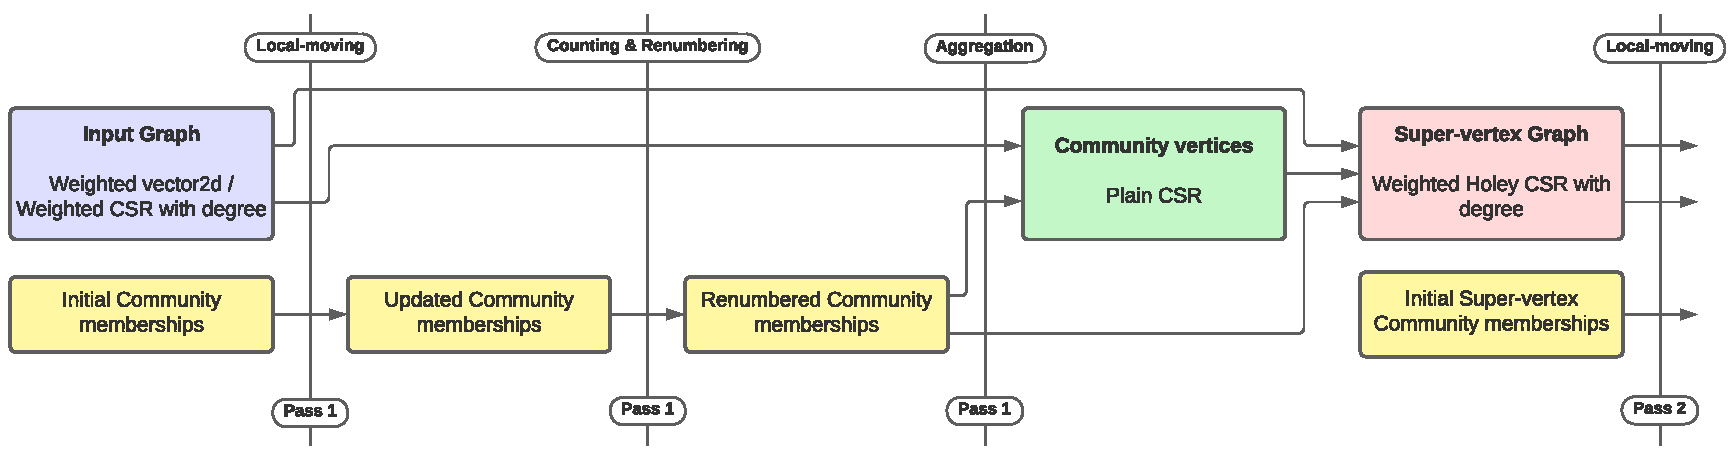
\includegraphics[width=0.98\linewidth]{out/louvain-pass.pdf}
  } \\[-2ex]
  \caption{A flow diagram illustrating the first pass of GVE-Louvain for a Weighted 2D-vector based or a Weighted CSR with degree based input graph. In the local-moving phase, vertex community memberships are updated until the total change in delta-modularity across all vertices reaches a specified threshold. Community memberships are then counted and renumbered. In the aggregation phase, community vertices in a CSR are first obtained. This is used to create the super-vertex graph stored in a Weighted Holey CSR with degree. In subsequent passes, the input is a Weighted Holey CSR with degree and initial community membership for super-vertices from the previous pass.}
  \label{fig:louvain-pass}
\end{figure*}
% A flow diagram showing the high level steps followed in the first pass of our Louvain implementation. The input graph is a weighted 2D vector based graph or weighted CSR with degree graph. In the local-moving phase, the community membership of each vertex is updated until the net change in delta-modularity across all vertices in an iteration reaches a threshold/tolerance. The community memberships are then counted and renumbered. In the aggregation phase of the algorithm, we obtain the vertices belonging to each community as a CSR, and later use this to generate the super-vertex graph. The super-vertex graph is stored in a weighted holey CSR with degree, i.e., the CSR is over-allocated with gaps between edges (ids and weights), and a degree vector is instead used to keep track of the degree of each super-vertex. In the remaining passes, the input graph is a weighted holey CSR with degree (from the previous pass) and an initial community membership vector for each super-vertex.